\documentclass[11pt,a4paper]{article}

\usepackage[margin=22mm,headheight=15pt]{geometry}
\usepackage[T1]{fontenc}
\usepackage{lmodern}
\usepackage{microtype}
\usepackage{amsmath,amssymb}
\usepackage{siunitx}
\usepackage{booktabs}
\usepackage{graphicx}
\usepackage{float}
\usepackage{enumitem}
\usepackage{xcolor}
\usepackage{caption}
\usepackage{fancyhdr}
\usepackage[hidelinks]{hyperref}

\definecolor{navy}{HTML}{17365D}
\definecolor{rulegray}{HTML}{B8C2CC}
\hypersetup{
  pdftitle={Saturation Temperature and Pressure Report 2026},
  pdfauthor={Aaron Taylor},
  pdfsubject={ENME 601 Thermodynamics Laboratory 1},
  pdfkeywords={saturation pressure, PT100, steam tables, thermodynamics}
}
\captionsetup{font=small,labelfont=bf,justification=centering}
\sisetup{round-mode=places,round-precision=2,detect-all}
\setlist[itemize]{leftmargin=6mm,itemsep=1.5pt,topsep=3pt}
\setlist[enumerate]{leftmargin=7mm,itemsep=2pt,topsep=3pt}
\setlength{\parindent}{0pt}
\setlength{\parskip}{4pt}
\setlength{\tabcolsep}{4.5pt}
\setlength{\emergencystretch}{1.5em}

\pagestyle{fancy}
\fancyhf{}
\fancyhead[L]{\small ENME 601 Thermodynamics}
\fancyhead[R]{\small Saturation Temperature and Pressure}
\fancyfoot[C]{\thepage}
\renewcommand{\headrulewidth}{0.4pt}
\newcommand{\sectionrule}{\vspace{-2pt}\color{rulegray}\hrule\color{black}\vspace{5pt}}

\begin{document}

\begin{center}
  {\LARGE\bfseries Saturation Temperature and Pressure Lab}\par
  \vspace{3mm}
  {\large Aaron Taylor --- 24232594}\par
  \vspace{1.5mm}
  {\large 1 August 2026}\par
\end{center}
\vspace{4mm}

\section*{Synopsis}
\sectionrule
The relationship between the saturation temperature and absolute pressure of
water was investigated using an Armfield TH3 saturation-pressure apparatus.
Nine equilibrium-stage readings were recorded from \SI{50}{\kilo\pascal} to
\SI{450}{\kilo\pascal} gauge pressure. The measured atmospheric pressure of
\SI{101.65}{\kilo\pascal} was added to each gauge reading. The original PT100
resistance readings were processed in two stages using the Armfield manual:
the console indication was corrected with Data Sheet~1, then converted to
temperature with Data Sheet~2. Linear interpolation was used between adjacent
tabulated values.

Both the experimental and published steam-table data followed a smooth power
relationship of the form $T=AP^n$. The experimental fit was
$T=31.218P^{0.2527}$, compared with $T=31.019P^{0.2557}$ for the direct
steam-table values. Experimental temperatures were below point-specific
interpolated theoretical values at all nine pressures. The mean signed error
was $-1.03\%$, and the largest absolute error was $1.89\%$. The close exponents
and small errors indicate that the experiment reproduced both the form and
magnitude of the saturation relationship. The remaining differences are
consistent with the assumptions of complete air purging, thermal equilibrium
and valid linear interpolation, together with heat loss, probe lag and
instrument resolution. Repeated readings at each pressure would be required
to separate repeatability from systematic bias.

\section{Aim}
\sectionrule
To measure the relationship between the saturation temperature and absolute
pressure of water, determine an empirical power-law model, and assess the
accuracy of the apparatus by comparison with published saturated-water data.

\section{Theory and Data Processing}
\sectionrule
At liquid--vapour equilibrium, saturated liquid water and saturated steam have
one saturation temperature for a given absolute pressure. Increasing pressure
raises this temperature and produces a smooth, nonlinear saturation curve.
The electronic pressure reading was gauge pressure, therefore
\begin{equation}
  P_{\mathrm{abs}}=P_1+P_{\mathrm{atm}},
  \qquad P_{\mathrm{atm}}=\SI{101.65}{\kilo\pascal}.
  \label{eq:pressure}
\end{equation}

The PT100 processing was a correction and reference-table conversion, not a
new two-point calibration. Armfield Data Sheet~1 corrects the indicated
resistance for imbalance in the console resistance bridge. For an indicated
resistance $R_m$ between adjacent entries $R_{m,a}$ and $R_{m,b}$,
\begin{equation}
 R_c=R_{c,a}+\frac{R_m-R_{m,a}}{R_{m,b}-R_{m,a}}
 (R_{c,b}-R_{c,a}).
 \label{eq:bridge}
\end{equation}
Data Sheet~2 then relates corrected resistance to PT100 temperature. Linear
interpolation between adjacent corrected-resistance values was used:
\begin{equation}
 T_{\mathrm{exp}}=T_a+\frac{R_c-R_{c,a}}{R_{c,b}-R_{c,a}}(T_b-T_a).
 \label{eq:pt100}
\end{equation}
Data Sheet~1 explicitly permits interpolation. Data Sheet~2 instructs the user
to select the closest entry; interpolation across its $2\,{}^\circ\mathrm{C}$
increments was adopted here as a stated processing assumption to retain the
resolution of the recorded resistances and avoid rounding every result to the
nearest $2\,{}^\circ\mathrm{C}$.

Over the measured range, both datasets were represented by
\begin{equation}
  T_{\mathrm{sat}}=AP_{\mathrm{sat}}^n,
  \label{eq:power}
\end{equation}
where $A$ and $n$ were obtained by a log-space least-squares fit. Direct values
from saturated-water pressure Table A--5 were used for the comparison curve.
For the error calculation only, the theoretical temperature at each
experimental pressure was found by linear interpolation:
\begin{equation}
  T_{\mathrm{th}}=T_a+\frac{P_{\mathrm{abs}}-P_a}{P_b-P_a}(T_b-T_a).
  \label{eq:interpolation}
\end{equation}
The signed percentage error was
\begin{equation}
  \mathrm{Error}\ (\%)=\frac{T_{\mathrm{exp}}-T_{\mathrm{th}}}
  {T_{\mathrm{th}}}\times100.
  \label{eq:error}
\end{equation}

\section{Equipment}
\sectionrule
The equipment comprised an Armfield TH3 saturation-pressure apparatus with a
\SI{2.4}{\litre} boiler, sight glass, closed pipe loop, cartridge heaters,
control console, filling and pressure-relief valves, a PT100 platinum
resistance thermometer, electronic and Bourdon pressure gauges, a barometer,
and de-ionised water. The manual gives a normal operating range of
0--\SI{7}{\bar} gauge and a maximum allowable pressure of \SI{8}{\bar} gauge.

\begin{figure}[H]
  \centering
  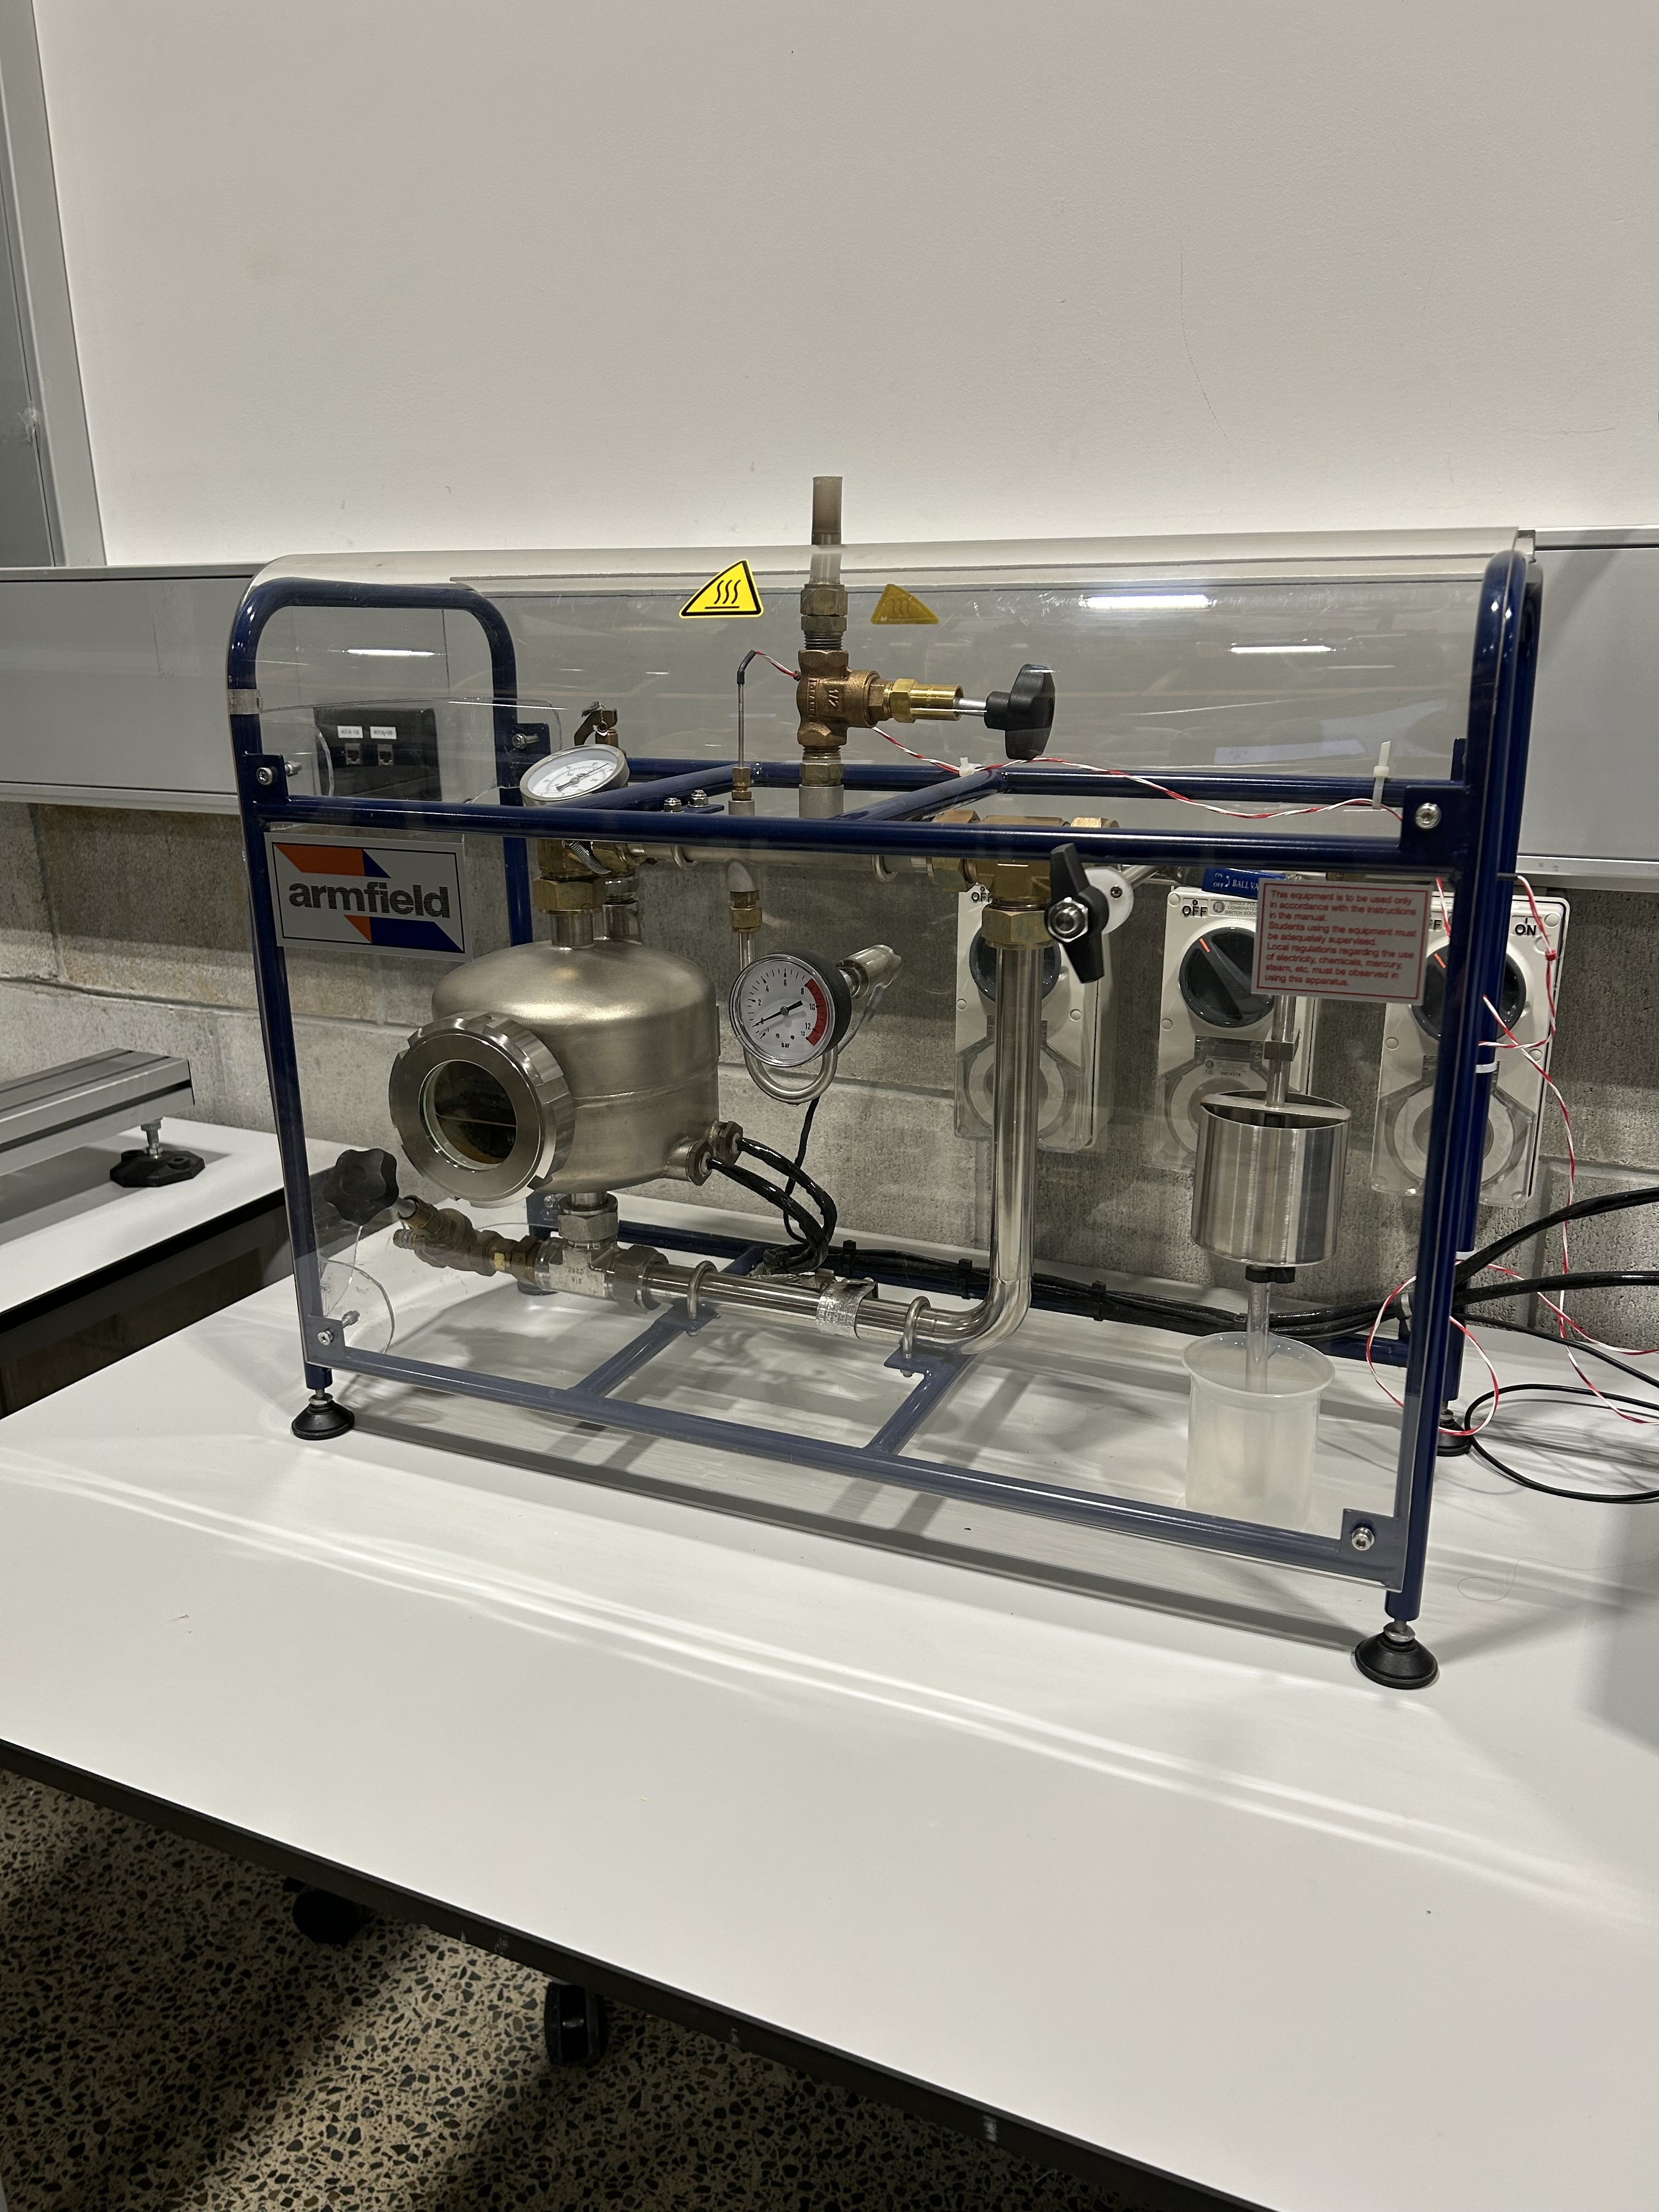
\includegraphics[width=0.90\textwidth,height=0.40\textheight,keepaspectratio]{Figure 1 - TH3 apparatus.jpeg}
  \caption{Armfield TH3 boiler and pipe loop used in the 2026 experiment. The
  photograph shows the boiler, pressure gauge, viewing port, valves and sensor
  wiring of the apparatus used.}
  \label{fig:apparatus}
\end{figure}

\section{Method}
\sectionrule
\begin{enumerate}
  \item With the drain and calorimeter isolating valves closed and console power
        off, the boiler was filled with de-ionised water to halfway up the sight glass.
  \item The water was heated to vigorous boiling with the filling point open.
        Steam was vented until the temperature indication stabilised, allowing air
        to be expelled from the loop.
  \item The filling valve was closed. The apparatus was then treated as a sealed,
        approximately constant-volume system containing a saturated water--steam
        mixture. Heater input was raised for approximately two minutes and reduced.
  \item Gauge pressure and PT100 resistance were recorded after the indication
        stabilised at nine stages from \SI{50}{\kilo\pascal} to
        \SI{450}{\kilo\pascal} gauge pressure.
  \item Gauge readings were converted to absolute pressure. Each indicated
        resistance was corrected using Armfield Data Sheet~1 and converted to
        temperature using Data Sheet~2.
  \item Experimental points and direct Table A--5 values were plotted on the same
        axes and fitted separately. Theoretical temperatures were then interpolated
        at the nine experimental pressures for the point-by-point error calculation.
  \item After the final reading, the heaters were switched off and the isolating
        valve was opened before cooling to prevent a damaging partial vacuum.
\end{enumerate}

\section{Results}
\sectionrule
\subsection{Worked calculation}
For the first reading, $P_1=\SI{50.00}{\kilo\pascal}$ and
$R_m=\SI{142.3}{\ohm}$:
\begin{align}
 P_{\mathrm{abs}}&=50.00+101.65=\SI{151.65}{\kilo\pascal},\\
 R_c&=142.32+\frac{142.3-142}{143-142}(143.54-142.32)
     =\SI{142.686}{\ohm}.
\end{align}
Data Sheet~2 gives $142.29~\Omega$ at $110\,{}^\circ\mathrm{C}$ and
$143.04~\Omega$ at $112\,{}^\circ\mathrm{C}$, therefore
\begin{align}
 T_{\mathrm{exp}}&=110+\frac{142.686-142.29}{143.04-142.29}(112-110)
 =111.056\,{}^\circ\mathrm{C},\\
 T_{\mathrm{th}}&=111.35+\frac{151.65-150}{175-150}(116.04-111.35)
 =111.660\,{}^\circ\mathrm{C},\\
 \mathrm{Error}&=\frac{111.056-111.660}{111.660}\times100=-0.541\%.
\end{align}

\subsection{Processed results}
\begin{table}[H]
  \centering
  \caption{Original measurements, Armfield PT100 conversion, theoretical temperatures and errors.}
  \label{tab:results}
  \small
  \begin{tabular}{rrrrrrr}
    \toprule
    $P_1$ & $P_{\mathrm{abs}}$ & $R_m$ & $R_c$ & $T_{\mathrm{exp}}$ & $T_{\mathrm{th}}$ & Error \\
    (kPa) & (kPa) & ($\Omega$) & ($\Omega$) & ($^\circ$C) & ($^\circ$C) & (\%) \\
    \midrule
     50 & 151.65 & 142.3 & 142.686 & 111.06 & 111.66 & $-0.54$ \\
    100 & 201.65 & 144.8 & 145.788 & 119.27 & 120.46 & $-0.98$ \\
    150 & 251.65 & 146.9 & 148.452 & 126.35 & 127.62 & $-0.99$ \\
    200 & 301.65 & 148.7 & 150.780 & 132.55 & 133.70 & $-0.86$ \\
    250 & 351.65 & 150.1 & 152.633 & 137.47 & 139.02 & $-1.11$ \\
    300 & 401.65 & 151.1 & 153.964 & 141.04 & 143.75 & $-1.89$ \\
    350 & 451.65 & 152.6 & 155.986 & 146.44 & 148.03 & $-1.07$ \\
    400 & 501.65 & 153.8 & 157.634 & 150.86 & 151.95 & $-0.71$ \\
    450 & 551.65 & 154.6 & 158.744 & 153.82 & 155.57 & $-1.12$ \\
    \bottomrule
  \end{tabular}
\end{table}

\subsection{Saturation curves and fitted equations}
Figure~\ref{fig:temperature} compares the processed experimental data with the
direct pressure--temperature pairs from Table A--5. Interpolated theoretical
points were not used to build either trendline.

\begin{figure}[H]
  \centering
  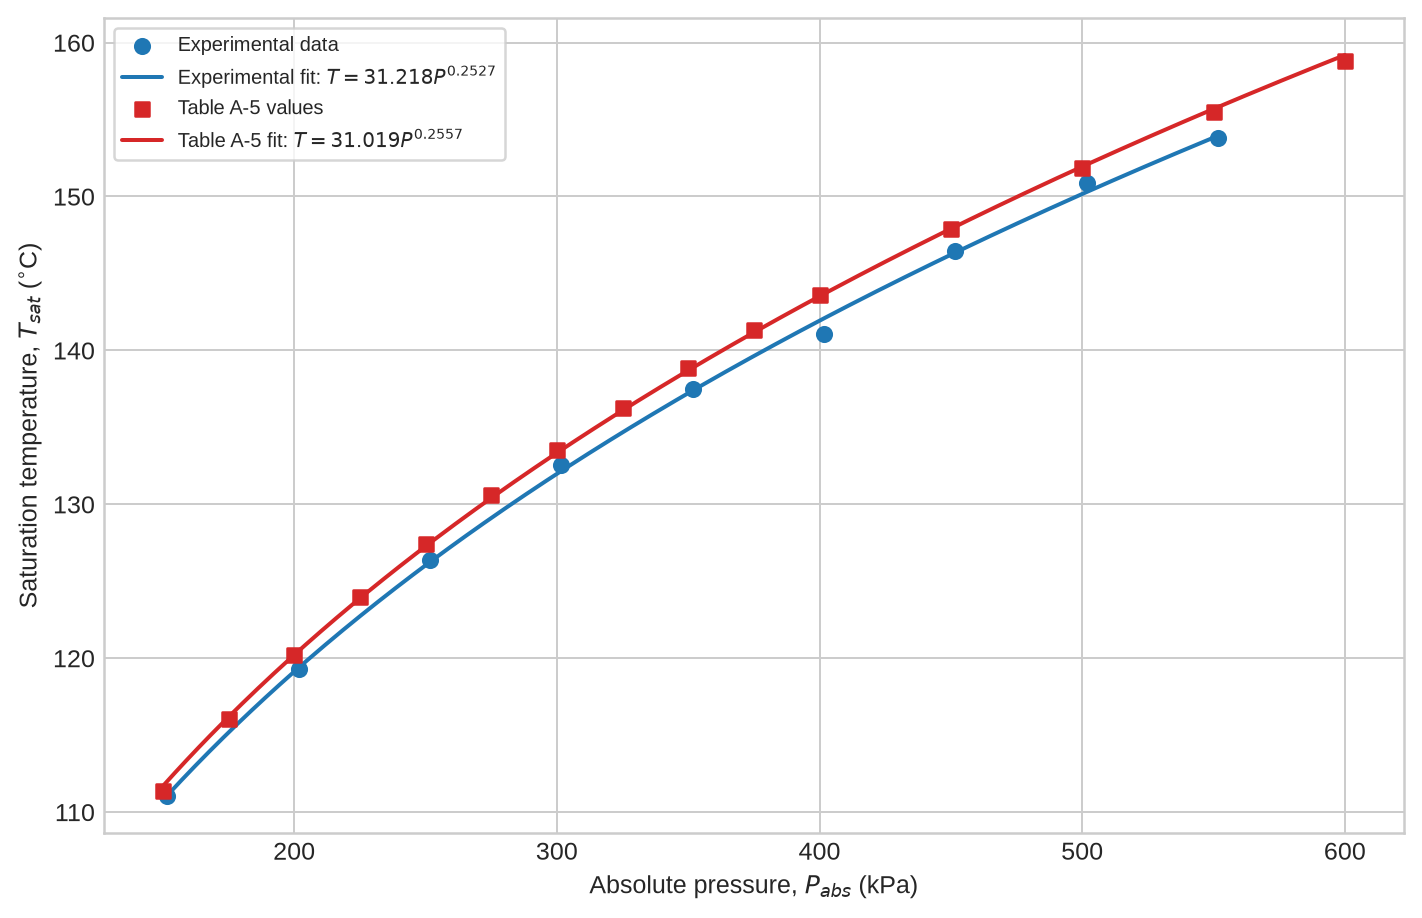
\includegraphics[width=0.78\textwidth]{Figure 2 v3 - Experimental and Table A5 values.png}
  \caption{Experimental temperatures and direct Table A--5 saturation values
  plotted against absolute pressure with separate power-law fits.}
  \label{fig:temperature}
\end{figure}

\begin{table}[H]
  \centering
  \caption{Power-law fit parameters for $T=AP^n$.}
  \label{tab:fits}
  \begin{tabular}{lrrr}
    \toprule
    Dataset & $A$ & $n$ & $R^2$ \\
    \midrule
    Experimental measurements & 31.218 & 0.2527 & 0.99904 \\
    Direct Table A--5 values & 31.019 & 0.2557 & 0.99983 \\
    \bottomrule
  \end{tabular}
\end{table}

\begin{figure}[H]
  \centering
  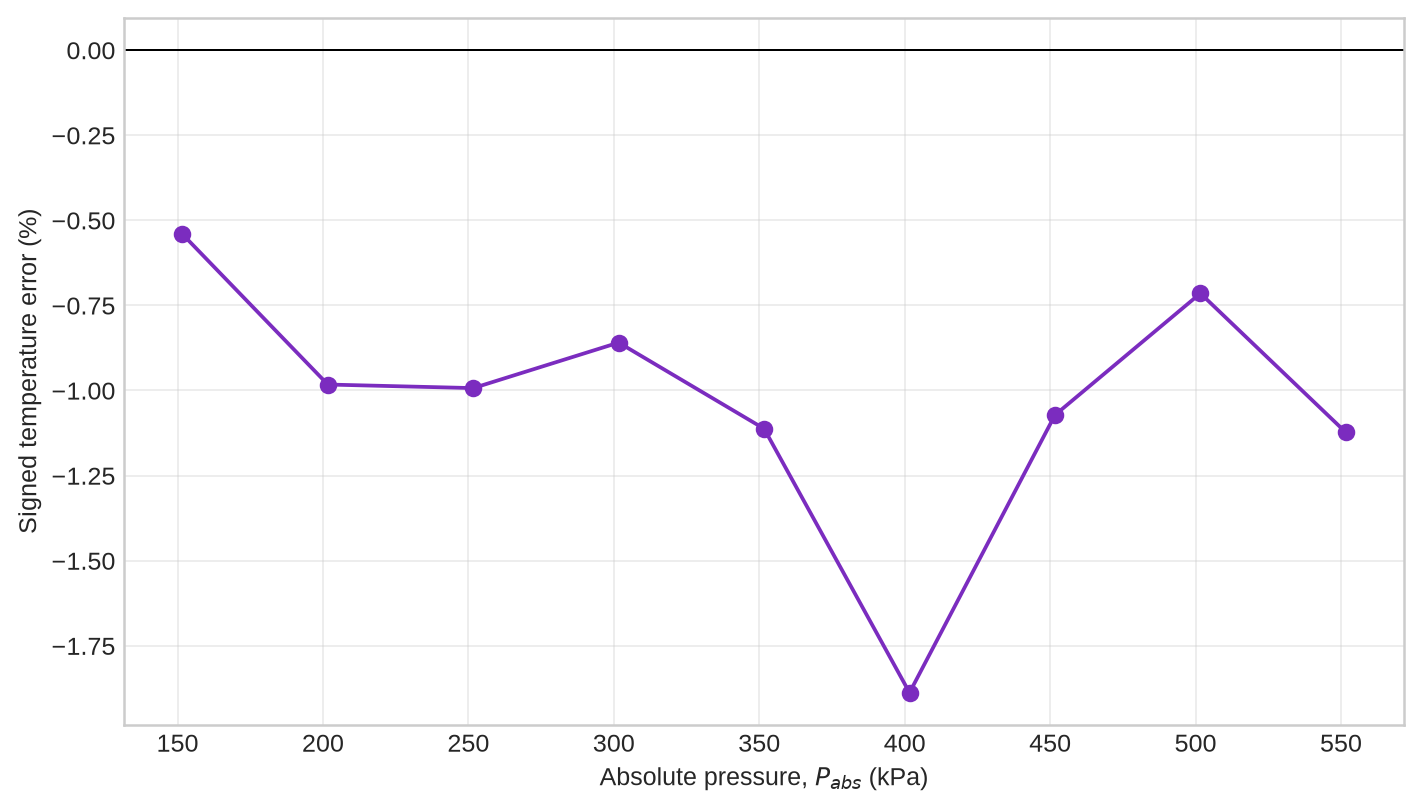
\includegraphics[width=0.56\textwidth]{Figure 3 v3 - Error versus absolute pressure.png}
  \caption{Signed experimental-temperature error relative to the point-specific
  interpolated saturation temperatures.}
  \label{fig:error}
\end{figure}

The mean signed error was $-1.03\%$. Since every value was below the reference,
the mean absolute error was also $1.03\%$. The maximum absolute error was
$1.89\%$ at \SI{401.65}{\kilo\pascal} absolute.

\section{Discussion}
\sectionrule
\subsection{Comparison and usefulness of the fitted equation}
The two curves increased smoothly with absolute pressure and had very similar
power-law parameters. The experimental exponent of 0.2527 differed from the
direct-table value of 0.2557 by only 0.0030. Both fits had $R^2>0.999$.
Therefore, the apparatus captured the expected nonlinear relationship and its
rate of increase over the measured range.

The experimental equation is useful as a compact empirical description of
these measurements between \SI{151.65}{\kilo\pascal} and
\SI{551.65}{\kilo\pascal} absolute. It should not replace steam tables in design
work or be extrapolated outside the tested interval because it depends on the
apparatus correction tables, measurement procedure and chosen fitting method.

\subsection{Error trend}
All signed errors were negative, indicating a small systematic tendency for the
measured temperature to lie below the reference saturation temperature. The
error did not increase monotonically with pressure: it ranged from $-0.54\%$ to
$-1.89\%$, peaked at \SI{401.65}{\kilo\pascal}, and then reduced. This pattern
supports a small negative bias combined with point-to-point experimental
variation, rather than a continuously growing pressure-dependent error.

\subsection{Steam temperature, water temperature and assumptions}
Saturated liquid and vapour have the same temperature only at thermodynamic
equilibrium. The PT100 measured steam in the upper pipework rather than liquid
inside the boiler. The comparison therefore made the following assumptions:
\begin{itemize}
  \item air was sufficiently purged for total measured pressure to approximate
        the steam saturation pressure;
  \item pressure, boiler water, local steam and the PT100 had reached a common
        equilibrium value before each reading;
  \item atmospheric pressure remained effectively constant during the run;
  \item linear interpolation between adjacent resistance and steam-table entries
        was adequate over the small intervals used; and
  \item the Armfield bridge-correction table represented the console and sensor
        used in the experiment.
\end{itemize}
These assumptions are reasonable for processing the data, but the experiment
did not test each one independently. Consequently, the possible causes below
are interpretations consistent with the observed errors, not proven mechanisms.

Thermal lag occurs because energy must conduct through the fluid, pipework and
probe sheath before the sensor reaches the local steam temperature. Heat loss
from exposed pipework can also keep the probe region slightly cooler than the
boiler. Either effect would produce negative temperature error if a reading were
taken before complete stabilisation.

\subsection{Possible sources of error and improvements}
\begin{itemize}
  \item \textbf{Residual air:} remaining non-condensable air contributes partial
        pressure, so the measured total pressure can exceed the steam partial
        pressure associated with the local saturation temperature.
  \item \textbf{Thermal lag and heat loss:} sensor response time and temperature
        gradients can make the upper-pipe measurement lower than the equilibrium
        boiler temperature.
  \item \textbf{Resistance conversion:} bridge correction, table resolution,
        rounding and linear interpolation influence every derived temperature.
  \item \textbf{Pressure measurement:} pressure-sensor calibration, display
        resolution and atmospheric-pressure uncertainty affect absolute pressure.
  \item \textbf{Single readings:} one value at each stage cannot distinguish
        random variation, hysteresis and repeatability from systematic bias.
\end{itemize}

The experiment would be stronger if each pressure stage were repeated after
independent stabilisation. Means and standard deviations could then be reported,
and an increasing-pressure run could be compared with a decreasing-pressure run
to identify hysteresis. Longer air purging, an explicit stability criterion for
both pressure and resistance, and documented instrument resolutions would
further strengthen the uncertainty assessment.

\section{Conclusion}
\sectionrule
The experiment reproduced the expected nonlinear increase in water saturation
temperature with absolute pressure. After the original resistance readings were
corrected and converted using the Armfield TH3 Data Sheets, the experimental
fit was $T=31.218P^{0.2527}$ with $R^2=0.99904$. This closely matched the direct
steam-table fit, $T=31.019P^{0.2557}$. Experimental temperatures were slightly
below point-specific theoretical values at all nine stages, with a mean signed
error of $-1.03\%$ and a maximum absolute error of $1.89\%$. The small negative
bias is consistent with assumptions concerning air purging and equilibrium and
with possible thermal lag, heat loss and instrument uncertainty. Repeated
measurements are recommended to quantify repeatability and determine whether
the remaining bias is systematic.

\section*{References}
{\footnotesize
\begin{enumerate}[itemsep=0pt,topsep=2pt]
  \item Y. A. \c{C}engel, M. A. Boles, and M. Kano\u{g}lu,
  \emph{Thermodynamics: An Engineering Approach}, 9th SI ed., McGraw-Hill,
  2020, Table A--5.
  \item Armfield Ltd., \emph{TH3 Saturation Pressure Apparatus Instruction Manual},
  Issue 15, Data Sheets 1--2, pp. 22--24.
  \item Auckland University of Technology, \emph{ENME 601 Saturation Temperature
  \& Pressure Lab Instructions}, 2025 update used for the 2026 laboratory.
\end{enumerate}
}

\end{document}
